\documentclass[a4paper,12pt]{article}

\usepackage{amsmath,amssymb,multicol,tikz,enumitem}
\usepackage[margin=2cm]{geometry}
\usetikzlibrary{calc,shapes}

\pagestyle{empty}

\newcommand\Q{\mathbf{Q}}
\newcommand\R{\mathbf{R}}
\newcommand\Z{\mathbf{Z}}

\usepackage{array}
\newcolumntype{P}[1]{>{\centering\arraybackslash}p{#1}}
\newcommand\indd{${}$\hspace{20pt}}

\begin{document}

\begin{center}
\parbox{3.5cm}{\textbf{Data Structures}} \hfill {\bf\Huge Worksheet 2} \hfill \parbox{3.5cm}{\flushright\textbf{BITL2}} \\[5pt]
\rm\small 9 September 2021
\end{center}

\hrule\vspace{2pt}\hrule

\begin{enumerate}

\item \textbf{Warm up:} Answer the following True / False questions.
\begin{enumerate}
\item Several pointers can point to the same \texttt{int}
\item One pointer can point to several \texttt{int}s
\item It is possible to create an array that holds both \texttt{int} and \texttt{char} types.  
\item It is possible to create an array that holds pointers to either both \texttt{int} or \texttt{char} types. 
\end{enumerate}
\end{enumerate}

\noindent
The next two problems refer to the following uncompiled \texttt{C++} files.
\[
\scalebox{.6}{ 
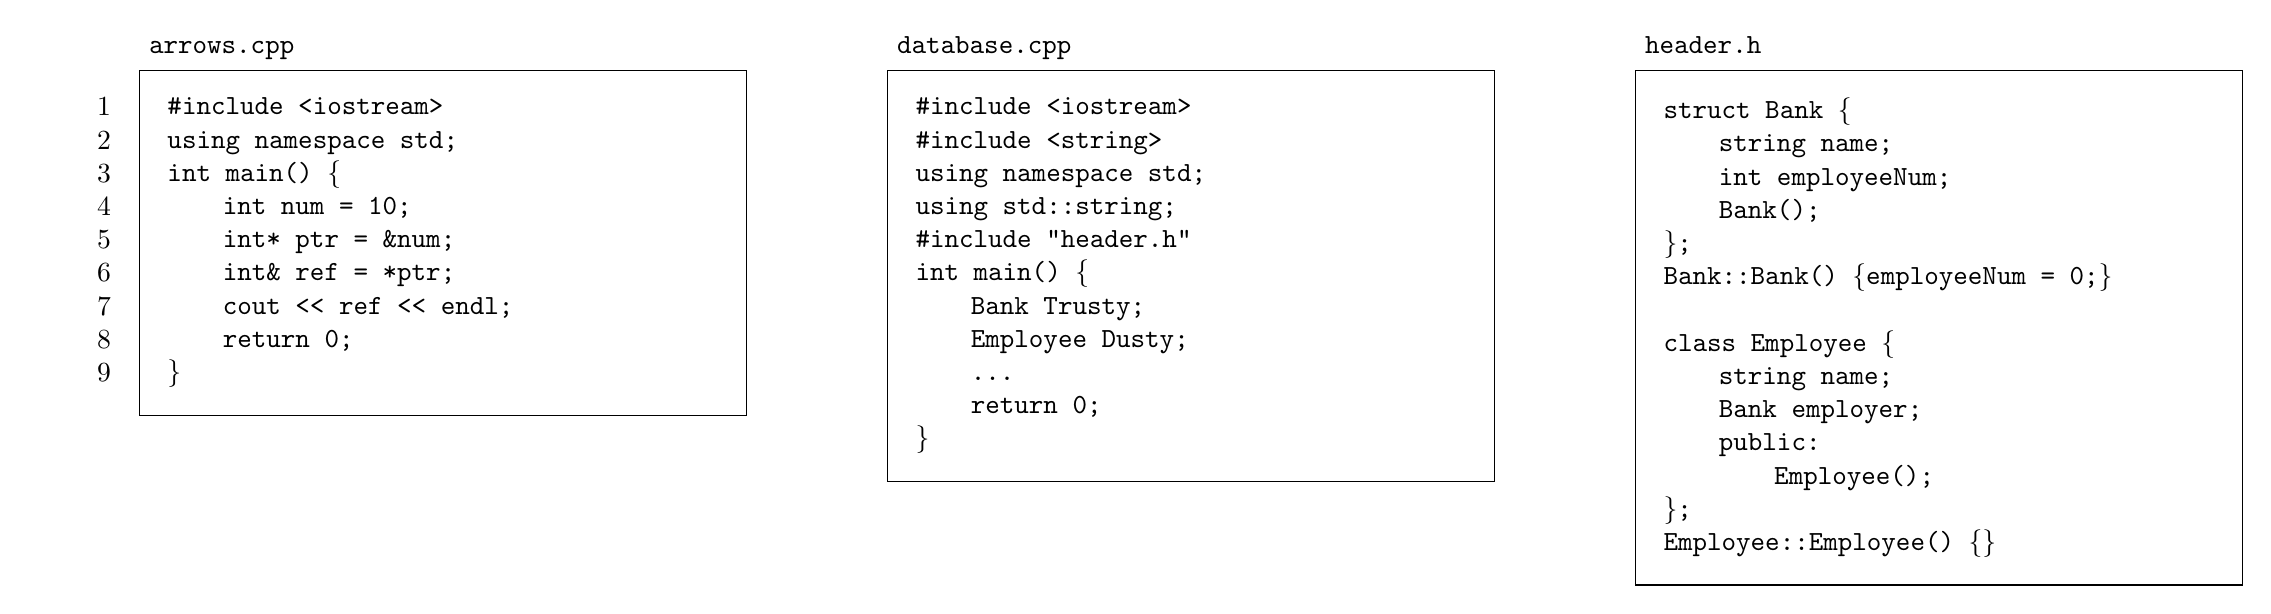
\begin{tikzpicture}
\node[draw,anchor=north,inner sep=10pt] (arrows) at (-10,0) {\parbox{7cm}{\raggedright
\texttt{\#include <iostream>}\linebreak
\texttt{using namespace std;}\linebreak
\texttt{int main() \{}\linebreak
\indd\texttt{int num = 10;}\linebreak
\indd\texttt{int* ptr = \&num;}\linebreak
\indd\texttt{int\& ref = *ptr;}\linebreak
\indd\texttt{cout << ref << endl;}\linebreak
\indd\texttt{return 0;}\linebreak
\texttt{\}}
}};
\node[anchor=south west] at (arrows.north west) {\texttt{arrows.cpp}};
\node[draw=white,anchor=north,inner sep=10pt,anchor=north east] at (arrows.north west) {\parbox{.7cm}{\raggedleft
1\linebreak 2\linebreak 3\linebreak 4\linebreak 5\linebreak 6\linebreak 7\linebreak 8\linebreak 9\linebreak}};


\node[draw,anchor=north,inner sep=10pt] (cpp) at (-.5,0) {\parbox{7cm}{\raggedright
\texttt{\#include <iostream>}\linebreak
\texttt{\#include <string>}\linebreak
\texttt{using namespace std;}\linebreak
\texttt{using std::string;}\linebreak
\texttt{\#include "header.h"}\linebreak
\texttt{int main() \{}\linebreak
\indd\texttt{Bank Trusty;}\linebreak
\indd\texttt{Employee Dusty;}\linebreak
\indd\texttt{...}\linebreak
\indd\texttt{return 0;}\linebreak
\texttt{\}}
}};
\node[anchor=south west] at (cpp.north west) {\texttt{database.cpp}};


\node[draw,anchor=north,inner sep=10pt] (head) at (9,0) {\parbox{7cm}{\raggedright
\texttt{struct Bank \{}\linebreak
\indd\texttt{string name;} \linebreak
\indd\texttt{int employeeNum;} \linebreak
\indd\texttt{Bank();} \linebreak
\texttt{\};}\linebreak
\texttt{Bank::Bank() \{employeeNum = 0;\}}\linebreak
%	bool isOpen;
%	int employeeNum;
%	void hired(int x);
%	void fired(int x);
%	Bank();
%//	Bank(string nm, bool op, int en = 0);
%};
\linebreak
\texttt{class Employee \{}\linebreak
\indd\texttt{string name;} \linebreak
\indd\texttt{Bank employer;} \linebreak
\indd\texttt{public:} \linebreak
\indd\indd\texttt{Employee();} \linebreak
\texttt{\};}\linebreak
\texttt{Employee::Employee() \{\}}
}};
\node[anchor=south west] at (head.north west) {\texttt{header.h\vphantom{p}}};
\end{tikzpicture}
}
\]

\begin{enumerate}
\item This question is about the program that results from compiling \texttt{arrows.cpp}.
\begin{enumerate}
\item What is the output of the program?
\item Change line 7 so that the output is the address of \texttt{num}.
\item What would happen (if anything) if the reference \texttt{ref} instead of the pointer \texttt{ptr} was defined first? That is, what will happend if lines 5 and 6 are replaced with:
%{\fontsize{9}{10}\selectfont
\begin{verbatim}
5       int& ref = *num;
6       int* ptr = &ref;
\end{verbatim}
%}
\item Suppose lines 6 and 7 are changed to 
\begin{verbatim}
6       int** newptr = &ptr;
7       cout << newptr << endl;
\end{verbatim}
What will be the output? How can you change this line 7 so that the output is \texttt{10}?
\end{enumerate}

\vfill

\item This question is about \texttt{database.cpp} and \texttt{header.h}.
\begin{enumerate}
\item For each the following options to place in the line \texttt{...} of \texttt{database.cpp}, decide wether or not an error will be produced when the file is compiled. If no error is produced, what will be the ouput when the resulting program is executed?
\begin{enumerate}
\item \texttt{cout << Trusty.employeeNum << endl;}
\item \texttt{cout << Trusty.name << endl;}
\item \texttt{Dusty.name = "Gutsy";}
\item \texttt{Trusty.name = "Musty"; cout << \&Trusty.name << endl;}
\item \texttt{Dusty.employer = Trusty; Dusty.employer.employeeNum++;}
\end{enumerate}
\item Create new public functions \texttt{setName} and \texttt{getName}, with constructors, for the class \texttt{Employee} that set the string \texttt{name} and that return it, respectively.
\end{enumerate}
\end{enumerate}

\end{document}